\documentclass[12pt, a4paper, oneside, openright, titlepage]{book}
\usepackage[utf8]{inputenc}
\raggedbottom
%%%%%%%%%%%%%%%%% Book Formatting Comments:

%%%%%%%%%%%%%%%%%%%%%%%%%%%%%%%%%%%%% for Part

%%%%%%%%%%%%%%%%%%%%%% for chapter

%%%%%%%%%%%%%%%%%%%% for section




%%%%%% PACKAGES %%%%%%%
\usepackage{hyperref}
\hypersetup{
    colorlinks,
    citecolor=black,
    filecolor=black,
    linkcolor=black,
    urlcolor=black
}
\usepackage{amsmath} % Math display options
\usepackage{amssymb} % Math symbols
%\usepackage{amsfonts} % Math fonts
%\usepackage{amsthm}
\usepackage{mathtools} % General math tools
\usepackage{array} % Allows you to write arrays
\usepackage{empheq} % For boxing equations
% \usepackage{mathabx}
% \usepackage{mathrsfs}
\usepackage{nameref}
\usepackage{wrapfig}

\usepackage{soul}
\usepackage[normalem]{ulem}

\usepackage{txfonts}
\usepackage{cancel}
\usepackage[toc, page]{appendix}
\usepackage{titletoc,tocloft}
\setlength{\cftchapindent}{1em}
\setlength{\cftsecindent}{2em}
\setlength{\cftsubsecindent}{3em}
%\setlength{\cftsubsubsecindent}{4em}
\usepackage{titlesec}

%\titleformat{\section}
%  {\normalfont\fontsize{25}{15}\bfseries}{\thesection}%{1em}{}
%\titleformat{\section}
%  {\normalfont\fontsize{20}{15}\bfseries}%{\thesubsection}{1em}{}
%\setcounter{secnumdepth}{1}  
  
  

%\newcommand\numberthis{\refstepcounter{equation}\tag{\theequation}} % For equation labelling
\usepackage[framemethod=tikz]{mdframed}

\usepackage{tikz} % For drawing commutative diagrams
\usetikzlibrary{cd}
\usetikzlibrary{calc}
\tikzset{every picture/.style={line width=0.75pt}} %set default line width to 0.75p

\usepackage{datetime}
\usepackage[margin=1.5in]{geometry}
\setlength{\parskip}{1em}
\usepackage{makeidx}         % allows index generation
\usepackage{graphicx}       % standard LaTeX graphics tool
\usepackage{multicol}        % used for the two-column index
\usepackage[bottom]{footmisc}% places footnotes at page bottom

\usepackage{newtxtext}       % 
\usepackage{newtxmath}       % selects Times Roman as basic font
\usepackage{float}
\usepackage{fancyhdr}
\setlength{\headheight}{15pt} 
\pagestyle{fancy}
\lhead[\leftmark]{}
\rhead[]{\leftmark}

%\usepackage{enumitem}

\usepackage{url}
\allowdisplaybreaks

%%%%%% ENVIRONMENTS %%%
\definecolor{purp}{rgb}{0.29, 0, 0.51}
\definecolor{bloo}{rgb}{0, 0.13, 0.80}



%%\newtheoremstyle{note}% hnamei
%{3pt}% hSpace above
%{3pt}% hSpace belowi
%{}% hBody fonti
%{}% hIndent amounti
%{\itshape}% hTheorem head fonti
%{:}% hPunctuation after theorem headi
%{.5em}% hSpace after theorem headi
%{}% hTheorem head spec (can be left empty, meaning ‘normal’)i





% %%%%%%%%%%%%% THEOREM DEFINITIONS

\spnewtheorem{axiom}{Axiom}[chapter]{\bfseries}{\itshape}


\spnewtheorem{construction}{Construction}[chapter]{\bfseries}{\itshape}

\spnewtheorem{props}{Properties}[chapter]{\bfseries}{\itshape}


\renewcommand{\qedsymbol}{$\blacksquare$}


\numberwithin{equation}{section}

\newenvironment{qest}{
    \begin{center}
        \em
    }
    {
    \end{center}
    }

%%%%%% MACROS %%%%%%%%%
%% New Commands
\newcommand{\ip}[1]{\langle#1\rangle} %%% Inner product
\newcommand{\abs}[1]{\lvert#1\rvert} %%% Modulus
\newcommand\diag{\operatorname{diag}} %%% diag matrix
\newcommand\tr{\mbox{tr}\.} %%% trace
\newcommand\C{\mathbb C} %%% Complex numbers
\newcommand\R{\mathbb R} %%% Real numbers
\newcommand\Z{\mathbb Z} %%% Integers
\newcommand\Q{\mathbb Q} %%% Rationals
\newcommand\N{\mathbb N} %%% Naturals
\newcommand\F{\mathbb F} %%% An arbitrary field
\newcommand\ste{\operatorname{St}} %%% Steinberg Representation
\newcommand\GL{\mathbf{GL}} %%% General Linear group
\newcommand\SL{\mathbf{SL}} %%% Special linear group
\newcommand\gl{\mathfrak{gl}} %%% General linear algebra
\newcommand\G{\mathbf{G}} %%% connected reductive group
\newcommand\g{\mathfrak{g}} %%% Lie algebra of G
\newcommand\Hbf{\mathbf{H}} %%% Theta fixed points of G
\newcommand\X{\mathbf{X}} %%% Symmetric space X
\newcommand{\catname}[1]{\normalfont\textbf{#1}}
\newcommand{\Set}{\catname{Set}} %%% Category set
\newcommand{\Grp}{\catname{Grp}} %%% Category group
\newcommand{\Rmod}{\catname{R-Mod}} %%% Category r-modules
\newcommand{\Mon}{\catname{Mon}} %%% Category monoid
\newcommand{\Ring}{\catname{Ring}} %%% Category ring
\newcommand{\Topp}{\catname{Top}} %%% Category Topological spaces
\newcommand{\Vect}{\catname{Vect}_{k}} %%% category vector spaces'
\newcommand\Hom{\mathbf{Hom}} %%% Arrows

\newcommand{\map}[2]{\begin{array}{c} #1 \\ #2 \end{array}}

\newcommand{\Emph}[1]{\textbf{\ul{\emph{#1}}}}




%% Math operators
\DeclareMathOperator{\ran}{Im} %%% image
\DeclareMathOperator{\aut}{Aut} %%% Automorphisms
\DeclareMathOperator{\spn}{span} %%% span
\DeclareMathOperator{\ann}{Ann} %%% annihilator
\DeclareMathOperator{\rank}{rank} %%% Rank
\DeclareMathOperator{\ch}{char} %%% characteristic
\DeclareMathOperator{\ev}{\bf{ev}} %%% evaluation
\DeclareMathOperator{\sgn}{sign} %%% sign
\DeclareMathOperator{\id}{Id} %%% identity
\DeclareMathOperator{\supp}{Supp} %%% support
\DeclareMathOperator{\inn}{Inn} %%% Inner aut
\DeclareMathOperator{\en}{End} %%% Endomorphisms
\DeclareMathOperator{\sym}{Sym} %%% Group of symmetries


%% Diagram Environments
\iffalse
\begin{center}
    \begin{tikzpicture}[baseline= (a).base]
        \node[scale=1] (a) at (0,0){
          \begin{tikzcd}
           
          \end{tikzcd}
        };
    \end{tikzpicture}
\end{center}
\fi




\newdateformat{monthdayyeardate}{%
    \monthname[\THEMONTH]~\THEDAY, \THEYEAR}
%%%%%%%%%%%%%%%%%%%%%%%



%%%%%% BEGIN %%%%%%%%%%


\begin{document}

%%%%%% TITLE PAGE %%%%%

\begin{titlepage}
    \centering
    \scshape
    \vspace*{\baselineskip}
    \rule{\textwidth}{1.6pt}\vspace*{-\baselineskip}\vspace*{2pt}
    \rule{\textwidth}{0.4pt}
    
    \vspace{0.75\baselineskip}
    
    {\LARGE Differential Geometry: A Complete Guide}
    
    \vspace{0.75\baselineskip}
    
    \rule{\textwidth}{0.4pt}\vspace*{-\baselineskip}\vspace{3.2pt}
    \rule{\textwidth}{1.6pt}
    
    \vspace{2\baselineskip}
    Subject \\
    \vspace*{3\baselineskip}
    \monthdayyeardate\today \\
    \vspace*{5.0\baselineskip}
    
    {\scshape\Large Elijah Thompson, \\ Physics and Math Honors\\}
    
    \vspace{1.0\baselineskip}
    \textit{Solo Pursuit of Learning}
    \vfill
    \enlargethispage{1in}
    \begin{figure}[b!]
    \makebox[\textwidth]{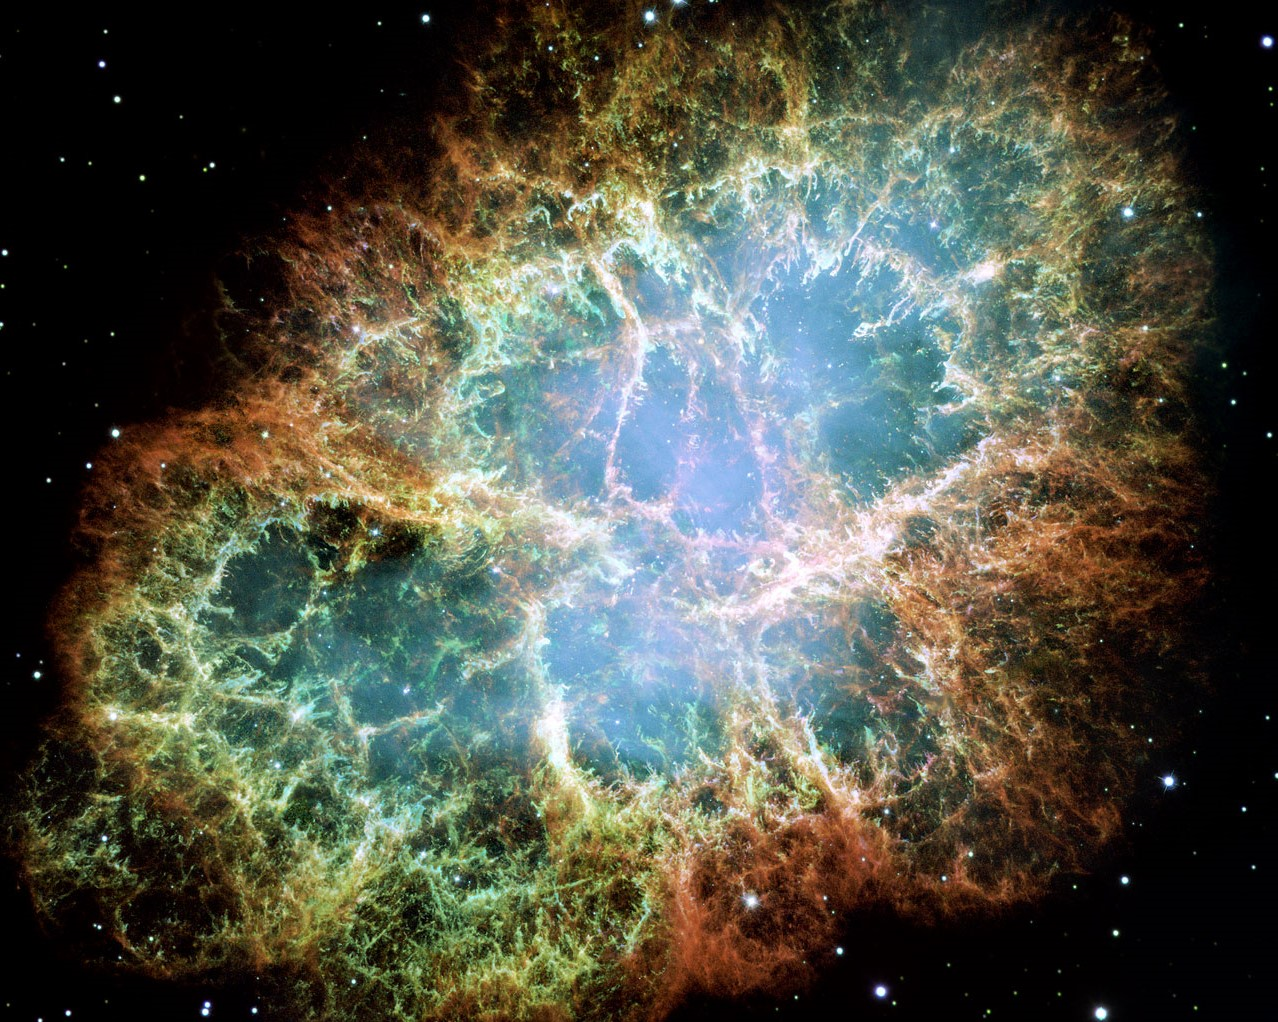
\includegraphics[width=\paperwidth, height =10cm]{../../Crab.jpg}}
    \end{figure}
\end{titlepage}

%%%%%%%%%%%%%%%%%%%%%%%
\tableofcontents

%%%%%%%%%%%%%%%%%%%%%%%%%%%%%%%%%%%%% Part 1
\part{Euclidean Geometry}

%%%%%%%%%%%%%%%%%%%%%% - P1.Chapter 1
\chapter{Postulates}

\section{Euclid's Postulates}



\begin{namthm}{Euclid's Postulates}
    \leavevmode
    \begin{enumerate}
        \item To draw a straight line, from any point to any point.
        \item To produce a finite straight line continuously in a straight line.
        \item To describe a \Emph{circle} with any center and distance.
        \item That all right angles are \Emph{equal} to another.
        \item That, if a straight line falling on two straight lines make the interior angles on the same side less than two right angles [in sum], then the two straight lines if produced indefinitely meet in that side on which the angles less than right angles.
        \begin{center}
            \begin{tikzpicture}[x=0.75pt,y=0.75pt,yscale=-0.8,xscale=0.8]
            %uncomment if require: \path (0,288); %set diagram left start at 0, and has height of 288
            
            %Straight Lines [id:da9956401651316147] 
            \draw    (80,199) -- (376,123) ;
            %Straight Lines [id:da5294043380028091] 
            \draw    (93,59) -- (398,172) ;
            %Straight Lines [id:da11513063298828397] 
            \draw    (230.33,40.67) -- (161,247.33) ;
            %Shape: Arc [id:dp06122376112034811] 
            \draw  [draw opacity=0] (215.96,84.06) .. controls (217.31,84.33) and (218.65,84.87) .. (219.94,85.69) .. controls (226.14,89.64) and (228.68,98.58) .. (225.6,105.68) .. controls (225.22,106.55) and (224.77,107.36) .. (224.27,108.09) -- (214.36,98.53) -- cycle ; \draw   (215.96,84.06) .. controls (217.31,84.33) and (218.65,84.87) .. (219.94,85.69) .. controls (226.14,89.64) and (228.68,98.58) .. (225.6,105.68) .. controls (225.22,106.55) and (224.77,107.36) .. (224.27,108.09) ;
            %Shape: Arc [id:dp5969785230152183] 
            \draw  [draw opacity=0] (191.37,156.12) .. controls (194.24,158.03) and (196.52,160.95) .. (197.62,164.57) .. controls (198.03,165.9) and (198.25,167.24) .. (198.31,168.56) -- (183.64,168.85) -- cycle ; \draw   (191.37,156.12) .. controls (194.24,158.03) and (196.52,160.95) .. (197.62,164.57) .. controls (198.03,165.9) and (198.25,167.24) .. (198.31,168.56) ;
            \end{tikzpicture}
        \end{center}
    \end{enumerate}
\end{namthm}

\begin{namthm}[Playfair's Postulate]
    This postulate is equivalent to Euclid's fifth postulate: Given straight line $m$ and point $P$ not on $m$, there exists a unique line $n$ that contains $P$ and is parallel to $m$.
\end{namthm}

\subsection{Hyperbolic Geometry Introduction}

\begin{defn}[Hyperbolic Plane]
    We define the hyperbolic plane to be the set \begin{equation}
        \mathcal{H} := \{(x,y) \in \R^2:y>0\}
    \end{equation}
    The hyperbolic metric is defined as \begin{equation}
        d_{\mathcal{H}}(\gamma) = \int_{\gamma}\frac{\sqrt{dx^2+dy^2}}{y}
    \end{equation}
    where $\gamma$ is a curve.
\end{defn}

\begin{prop}
    \leavevmode
    \begin{center}
        \begin{tikzpicture}[x=0.75pt,y=0.75pt,yscale=-1,xscale=1]
        %uncomment if require: \path (0,300); %set diagram left start at 0, and has height of 300
        
        %Straight Lines [id:da2992176096767445] 
        \draw    (70.25,160.25) -- (298.25,159.75) ;
        \draw [shift={(300.25,159.75)}, rotate = 539.88] [color={rgb, 255:red, 0; green, 0; blue, 0 }  ][line width=0.75]    (10.93,-3.29) .. controls (6.95,-1.4) and (3.31,-0.3) .. (0,0) .. controls (3.31,0.3) and (6.95,1.4) .. (10.93,3.29)   ;
        %Shape: Circle [id:dp3110941479285647] 
        \draw   (139.96,160.41) .. controls (139.96,138.15) and (158.01,120.11) .. (180.27,120.11) .. controls (202.53,120.11) and (220.57,138.15) .. (220.57,160.41) .. controls (220.57,182.67) and (202.53,200.71) .. (180.27,200.71) .. controls (158.01,200.71) and (139.96,182.67) .. (139.96,160.41) -- cycle ;
        %Shape: Arc [id:dp5032500480592332] 
        \draw  [draw opacity=0] (190.74,150.15) .. controls (193.16,152.47) and (194.68,155.66) .. (194.74,159.21) -- (181.09,159.46) -- cycle ; \draw   (190.74,150.15) .. controls (193.16,152.47) and (194.68,155.66) .. (194.74,159.21) ;
        %Shape: Arc [id:dp13509255220922078] 
        \draw  [draw opacity=0] (182.66,149.06) .. controls (187.94,150.13) and (191.94,154.68) .. (192.04,160.19) -- (180.27,160.41) -- cycle ; \draw   (182.66,149.06) .. controls (187.94,150.13) and (191.94,154.68) .. (192.04,160.19) ;
        %Shape: Arc [id:dp2607850656819486] 
        \draw  [draw opacity=0] (189.05,121.09) .. controls (196.74,122.81) and (203.6,126.72) .. (208.94,132.12) -- (180.14,160.41) -- cycle ; \draw  [color={rgb, 255:red, 241; green, 13; blue, 13 }  ,draw opacity=1 ] (189.05,121.09) .. controls (196.74,122.81) and (203.6,126.72) .. (208.94,132.12) ;
        %Straight Lines [id:da7840961832979934] 
        \draw    (189.14,120.71) -- (180.27,160.41) ;
        \draw [shift={(180.27,160.41)}, rotate = 102.6] [color={rgb, 255:red, 0; green, 0; blue, 0 }  ][fill={rgb, 255:red, 0; green, 0; blue, 0 }  ][line width=0.75]      (0, 0) circle [x radius= 1.34, y radius= 1.34]   ;
        \draw [shift={(189.14,120.71)}, rotate = 102.6] [color={rgb, 255:red, 0; green, 0; blue, 0 }  ][fill={rgb, 255:red, 0; green, 0; blue, 0 }  ][line width=0.75]      (0, 0) circle [x radius= 1.34, y radius= 1.34]   ;
        %Straight Lines [id:da9255161199383619] 
        \draw [fill={rgb, 255:red, 19; green, 18; blue, 18 }  ,fill opacity=1 ]   (208.94,132.12) -- (180.27,160.41) ;
        \draw [shift={(180.27,160.41)}, rotate = 135.39] [color={rgb, 255:red, 0; green, 0; blue, 0 }  ][fill={rgb, 255:red, 0; green, 0; blue, 0 }  ][line width=0.75]      (0, 0) circle [x radius= 1.34, y radius= 1.34]   ;
        \draw [shift={(208.94,132.12)}, rotate = 135.39] [color={rgb, 255:red, 0; green, 0; blue, 0 }  ][fill={rgb, 255:red, 0; green, 0; blue, 0 }  ][line width=0.75]      (0, 0) circle [x radius= 1.34, y radius= 1.34]   ;
        
        % Text Node
        \draw (196.04,150.14) node [anchor=north west][inner sep=0.75pt]  [font=\tiny,rotate=-1.53,xslant=0]  {$\alpha $};
        % Text Node
        \draw (186.17,140.7) node [anchor=north west][inner sep=0.75pt]  [font=\tiny]  {$\beta $};
        % Text Node
        \draw (179.5,106.9) node [anchor=north west][inner sep=0.75pt]  [font=\scriptsize]  {$Q$};
        % Text Node
        \draw (212.17,121.23) node [anchor=north west][inner sep=0.75pt]  [font=\scriptsize]  {$P$};
        % Text Node
        \draw (197.17,111.9) node [anchor=north west][inner sep=0.75pt]  [font=\tiny]  {$\gamma _{Q,P}$};
        % Text Node
        \draw (170.5,163.23) node [anchor=north west][inner sep=0.75pt]  [font=\tiny]  {$( C,0)$};
        \end{tikzpicture}
    \end{center}
    For $\alpha < \beta$ we have that \begin{equation}
        d_{\mathcal{H}}(\gamma_{Q,P}) = \ln\left[\frac{\csc\beta - \cot\beta}{\csc\alpha - \cot\alpha}\right]
    \end{equation}
    Moreover, if we had a line segment from $(a,y_1)$ to $(a,y_2)$, the hyperbolic length would be \begin{equation}
        d_{\mathcal{H}}(l) = \int_{l}\frac{1}{y}\sqrt{\frac{dx}{dt}^2+\frac{dy}{dt}^2}dt = \int_{y_1}^{y_2}\frac{1}{t}dt = \ln\left(\frac{y_2}{y_1}\right)
    \end{equation}
\end{prop}

\begin{prop}
    Euclidean angles are the same as hyperbolic angles.
\end{prop}

\begin{qest}
    What is a line?
\end{qest}
\begin{enumerate}
    \item[$\drsh$] A line is a \Emph{geodesic}, which is the shortest path with respect to the metric of the geometry (the distance function). 
\end{enumerate}
\begin{thm}
    In the hyperbolic plane the geodesics are either vertical lines (rays from the Euclidean respective), or semi-circles, terminating asymptotically to the $x$-axis.
\end{thm}

\begin{rmk}
    Given a circle with center $(h,k)$ above the $x$-axis in the Euclidean plane, the image in the hyperbolic plane is a circle centered at $(H,K)$ with $H = \sqrt{k^2-r^2}$, $R = \frac{1}{2}\ln\left(\frac{k+r}{k-r}\right)$, and $K = k$.
\end{rmk}

\begin{rmk}
    The hyperbolic half-plane satisfies Euclid's first four axioms, but the fifth (e.i Playfair's Postulate) is not satisfied in the hyperbolic half-plane. 
\end{rmk}

%%%%%%%%%%%%%%%%%%%%%% - P1.Chapter 2
\chapter{Tangent and Normal Spaces}

\section{Notation}

\begin{rmk}
    In $\R^n$ we shall write $(p+q)^i = p^i+q^i$ (component wise addition) with $i$ as an index and $(cp)^i = cp^i$. For $p \in \R^n$ we have\begin{align*}
        p &= (p^1,p^2,...,p^n) \\
        &=p^1(1,0,...,0) + p^2(0,1,...,0) + ... + p^n(0,...,0,1) \\
        &= \sum\limits_{i=1}^np^ie_i
    \end{align*}
    We define the \Emph{Kroneker Delta} to be \begin{equation}
        \delta_{ij} = \left\{\begin{array}{ll} 1 & \text{if } i = j \\ 0 & \text{if } i \neq j \end{array}\right.
    \end{equation}
\end{rmk}

\begin{rmk}
    There exists a correspondence between points and vectors based at the origin $(0,0,...,0)$.
\end{rmk}

\section{Definitions and Examples}

\begin{defn}
    The \Emph{tangent space} to $\R^n$ at a point $p \in \R^n$ is defined as \begin{equation}
        T_p\R^n :=\{p\}\times \R^n = \{(p,v):v\in\R^n\}
    \end{equation} 
    Then, the \Emph{tangent bundle} is defined as \begin{equation}
        T\R^n := \bigcup_{p \in \R^n}T_p\R^n
    \end{equation}
\end{defn}

\begin{rmk}
    We give $T_p\R^n$ a vector space structure by defining an addition \begin{equation}
        (p,v) + (p,w) := (p,v+w)
    \end{equation}
    for all $v,w \in \R^n$, and we define scalar multiplication by \begin{equation}
        c(p,v) = (p,cv)
    \end{equation}
    for all $c \in \R$. We can also define a standard inner product on $T_p\R^n$ by \begin{equation}
        (p,v) \cdot (p,w) = v\cdot w = v^Tw
    \end{equation}
    as well as a norm \begin{equation}
        ||(p,v)|| = ||v||
    \end{equation}
    We say that $(p,v),(p,w) \in T_P\R^n$ are orthogonal if \begin{equation}
        (p,v) \cdot (p,w) = 0 = v\cdot w
    \end{equation}
    Given a subspace $S \subset T_p\R^n$, we have the orthogonal complement of $S$ \begin{equation}
        S^{\perp} := \{(p,w) \in T_p\R^n: (p,w)\cdot (p,v) = 0,\forall (p,v) \in S\}
    \end{equation}
\end{rmk}


\begin{defn}
    For a curve $C$, we can define the tangent space at a point $p$ on $C$ by \begin{equation}
        T_pC := \spn\{(p,v)\} \subset T_p\R^n
    \end{equation}
    where $(p,v)$ is tangent to $C$ at $p$. Then, we have that \begin{equation}
        (T_pC)^{\perp} = \text{normal space to $C$ at $p$}
    \end{equation}
    For $n = 2$ we get the normal line, for $n = 3$ we get the normal plane, etc.
\end{defn}

\begin{eg}
    $\alpha(t) = (t,t^2)$, $p = \alpha(1) = (1,1)$. Then $\alpha'(1) = \langle 1,2\rangle$, so $v = (p,\langle 1, 2\rangle)$. This parametrizes a parabola in $\R^2$.
\end{eg}


%%%%%%%%%%%%%%%%%%%%%%%%%%%%%%%%%%%%% Part 2
\part{Manifold Theory}

%%%%%%%%%%%%%%%%%%%%%% - P2.Chapter 1
\chapter{Manifold Definitions and Types}


%%%%%%%%%%%%%%%%%%%%%% - P2.Chapter 2
\chapter{Smooth Maps}



%%%%%%%%%%%%%%%%%%%%%% - P2.Chapter 3
\chapter{Immersions, Submersions, and Submanifolds}



%%%%%%%%%%%%%%%%%%%%%% - P2.Chapter 4
\chapter{Tangent Bundles}


%%%%%%%%%%%%%%%%%%%%%% - P2.Chapter 5
\chapter{Differential Forms}



%%%%%%%%%%%%%%%%%%%%%% - P2.Chapter 6
\chapter{Integration on Manifolds}



%%%%%%%%%%%%%%%%%%%%%% - P2.Chapter 7
\chapter{Stoke's Theorem}







\end{document}


%%%%%% END %%%%%%%%%%%%%u
